%  The AAU Poster Theme.
%  2013-05-08 v. 1.1.0
%  Copyright 2013 by Jesper Kjær Nielsen <jkn@es.aau.dk>
%
%  This is free software: you can redistribute it and/or modify
%  it under the terms of the GNU General Public License as published by
%  the Free Software Foundation, either version 3 of the License, or
%  (at your option) any later version.
%
%  This is distributed in the hope that it will be useful,
%  but WITHOUT ANY WARRANTY; without even the implied warranty of
%  MERCHANTABILITY or FITNESS FOR A PARTICULAR PURPOSE.  See the
%  GNU General Public License for more details.
%
%  You can find the GNU General Public License at <http://www.gnu.org/licenses/>.
\documentclass[a0paper,landscape]{baposter}
%%%%%%%%%%%%%%%%%%%%%%%%%%%%%%%%%%%%%%%%%%%%%%%%
% Language, Encoding and Fonts
% http://en.wikibooks.org/wiki/LaTeX/Internationalization
%%%%%%%%%%%%%%%%%%%%%%%%%%%%%%%%%%%%%%%%%%%%%%%%
% Select encoding of your inputs. Depends on
% your operating system and its default input
% encoding. Typically, you should use
%   Linux  : utf8 (most modern Linux distributions)
%            latin1 
%   Windows: ansinew
%            latin1 (works in most cases)
%   Mac    : applemac
% Notice that you can manually change the input
% encoding of your files by selecting "save as"
% an select the desired input encoding. 
\usepackage[utf8]{inputenc}
% Make latex understand and use the typographic
% rules of the language used in the document.
\usepackage[english]{babel}
% Use the vector font Latin Modern which is going
% to be the default font in latex in the future.
\usepackage{helvet}
% Change the default font family from roman to sans serif
\renewcommand{\familydefault}{\sfdefault} % for text
\usepackage[helvet]{sfmath} % for math
% Choose the font encoding
\usepackage[T1]{fontenc}
\usepackage[font=small,labelfont=bf]{caption}
\DeclareCaptionFont{tiny}{\footnotesize}
\usepackage{enumitem}
%%%%%%%%%%%%%%%%%%%%%%%%%%%%%%%%%%%%%%%%%%%%%%%%
% Graphics and Tables
% http://en.wikibooks.org/wiki/LaTeX/Importing_Graphics
% http://en.wikibooks.org/wiki/LaTeX/Tables
% http://pgfplots.sourceforge.net/
%%%%%%%%%%%%%%%%%%%%%%%%%%%%%%%%%%%%%%%%%%%%%%%%
% You cannot use floats in the baposter theme.
% We therefore load the caption package which provides
% the command \captionof
% Set up how figure and table captions are displayed
\usepackage{caption}
\captionsetup{
  font=large,% set font size to footnotesize
  labelfont=bf % bold label (e.g., Figure 3.2) font
}
% Make the standard latex tables look so much better
\usepackage{array,booktabs}
% For creating beautiful plots
\usepackage{pgfplots}

\usepackage{graphicx}
\usepackage{nicefrac}
\usepackage{mathtools}
\usepackage{tabularx,booktabs,ragged2e}
\usepackage{xcolor}
%\usepackage{showframe}
\usepackage[framemethod=tikz]{mdframed}

%%%%%%%%%%%%%%%%%%%%%%%%%%%%%%%%%%%%%%%%%%%%%%%%
% Mathematics
% http://en.wikibooks.org/wiki/LaTeX/Mathematics
%%%%%%%%%%%%%%%%%%%%%%%%%%%%%%%%%%%%%%%%%%%%%%%%
% Defines new environments such as equation,
% align and split 
\usepackage{amsmath}
% Adds new math symbols
\usepackage{amssymb}

%%%%%%%%%%%%%%%%%%%%%%%%%%%%%%%%%%%%%%%%%%%%%%%%
% Colours
% http://en.wikibooks.org/wiki/LaTeX/Colors
%%%%%%%%%%%%%%%%%%%%%%%%%%%%%%%%%%%%%%%%%%%%%%%%
\selectcolormodel{RGB}
% define the three aau colors
\definecolor{aaublue1}{RGB}%
{33,26,82}
%{33,26,82}% dark blue
\definecolor{aaublue2}{RGB}{113,109,143} % light blue
\definecolor{aaublue3}{RGB}{194,193,204} % lighter blue

%%%%%%%%%%%%%%%%%%%%%%%%%%%%%%%%%%%%%%%%%%%%%%%%
% Lists
% http://en.wikibooks.org/wiki/LaTeX/List_Structures
%%%%%%%%%%%%%%%%%%%%%%%%%%%%%%%%%%%%%%%%%%%%%%%%

\usepackage{float}
\usepackage{caption}
\usepackage{subcaption}

\usepackage{pgfplots}
\usepackage{tikz}

% Easier configuration of lists
\usepackage{enumitem}
%configure itemize
\setlist{%
  topsep=0pt,% set space before and after list
  noitemsep,% remove space between items
  labelindent=\parindent,% set the label indentation to the paragraph indentation
  leftmargin=*,% remove the left margin
  font=\color{aaublue1}\normalfont, %set the colour of all bullets, numbers and descriptions to aaublue1
}
% use set<itemize,enumerate,description> if you have an older latex distribution
\setitemize[1]{label={\raise1.25pt\hbox{$\blacktriangleright$}}}
\setitemize[2]{label={\scriptsize\raise1.25pt\hbox{$\blacktriangleright$}}}
\setitemize[3]{label={\raise1.25pt\hbox{$\star$}}}
\setitemize[4]{label={-}}
%\setenumerate[1]{label={\theenumi.}}
%\setenumerate[2]{label={(\theenumii)}}
%\setenumerate[3]{label={\theenumiii.}}
%\setenumerate[4]{label={\theenumiv.}}
%\setdescription{font=\color{aaublue1}\normalfont\bfseries}

% use setlist[<itemize,enumerate,description>,<level>] if you have a newer latex distribution
%\setlist[itemize,1]{label={\raise1.25pt\hbox{$\blacktriangleright$}}}
%\setlist[itemize,2]{label={\scriptsize\raise1.25pt\hbox{$\blacktriangleright$}}}
%\setlist[itemize,3]{label={\raise1.25pt\hbox{$\star$}}}
%\setlist[itemize,4]{label={-}}
%\setlist[enumerate,1]{label={\theenumi.}}
%\setlist[enumerate,2]{label={(\theenumii)}}
%\setlist[enumerate,3]{label={\theenumiii.}}
%\setlist[enumerate,4]{label={\theenumiv.}}
%\setlist[description]{font=\color{aaublue1}\normalfont\bfseries}

%%%%%%%%%%%%%%%%%%%%%%%%%%%%%%%%%%%%%%%%%%%%%%%%
% Misc
%%%%%%%%%%%%%%%%%%%%%%%%%%%%%%%%%%%%%%%%%%%%%%%%
% change/remove some names
\addto{\captionsenglish}{
  %remove the title of the bibliograhpy
  \renewcommand{\refname}{\vspace{-0.7em}}
  %change Figure to Fig. in figure captions
  \renewcommand{\figurename}{Fig.}
}
% create links
\usepackage{url}
%note that the hyperref package is currently incompatible with the baposter class

%%%%%%%%%%%%%%%%%%%%%%%%%%%%%%%%%%%%%%%%%%%%%%%%
% Macros
%%%%%%%%%%%%%%%%%%%%%%%%%%%%%%%%%%%%%%%%%%%%%%%%
\newcommand{\alert}[1]{{\color{aaublue1}#1}}

\usepackage{tabularx} % in the preamble
\newcolumntype{Y}{>{\raggedright\arraybackslash}X}

\newcommand*\circled[1]{\tikz[baseline=(char.base)]{
            \node[shape=circle,fill=white, thick,inner sep=0.3pt,text=aaublue1] (char) {#1};}}
            
\newcommand*\titcleCirc[2]{\begin{tabularx}{\textwidth}{YcY}
 & #1 & \circled{#2}
  \end{tabularx}
}            
%%%%%%%%%%%%%%%%%%%%%%%%%%%%%%%%%%%%%%%%%%%%%%%%

% *** CITATION PACKAGES ***
  \usepackage[square, numbers, comma, sort&compress]{natbib}      
  \bibliographystyle{ieeetr}

%%%%%%%%%%%%%%%%%%%%%%%%%%%%%%%%%%%%%%%%%%%%%%%%
  
% Document Start 
%%%%%%%%%%%%%%%%%%%%%%%%%%%%%%%%%%%%%%%%%%%%%%%%
\begin{document}
%%%%%%%%%%%%%%%%%%%%%%%%%%%%%%%%%%%%%%%%%%%%%%%%
% Some changes that cannot be made in the preamble
%%%%%%%%%%%%%%%%%%%%%%%%%%%%%%%%%%%%%%%%%%%%%%%%
% set the background of the poster
\background{
  \begin{tikzpicture}[remember picture,overlay]%
    %the poster background color
    \fill[fill=aaublue3] (current page.north west) rectangle (current page.south east);
    %the header
    \fill [fill=aaublue1] (current page.north west) rectangle ([yshift=-\headerheight] current page.north east);
  \end{tikzpicture}
}
% if you want to reduce the space before and after equations, use and adjust
% the following lines
%\addtolength{\abovedisplayskip}{-2mm}
%\addtolength{\belowdisplayskip}{-2mm}

%%%%%%%%%%%%%%%%%%%%%%%%%%%%%%%%%%%%%%%%%%%%%%%%
% General poster setup
%%%%%%%%%%%%%%%%%%%%%%%%%%%%%%%%%%%%%%%%%%%%%%%%
\begin{poster}{
  %general options for the poster
  grid=false,
  columns=3,
%  colspacing=4.2mm,
  headerheight=0.1\textheight,
  background=user,
%  bgColorOne=red!42, %is used when background != user and none
%  bgColortwo=green!42, %is used when background is shaded
  eyecatcher=true,
  %posterbox options
  headerborder=closed,
  borderColor=aaublue1,
  headershape=rectangle,
  headershade=plain,
  headerColorOne=aaublue1,
%  headerColortwo=yellow!42, %is used when the header background is shaded
  textborder=rectangle,
  boxshade=plain,
  boxColorOne=white,
%  boxColorTwo=cyan!42,%is used when the text background is shaded
  headerFontColor=white,
  headerfont=\Large\sf\bf,
  linewidth=1pt
}
%the Eye Catcher (the logo on the left)
{
  %this can be commented out or replaced by a company/department logo
  
\includegraphics[height=0.75\headerheight]{aau_logo_new_neg}
}
%the poster title
{\color{white}\bf
  Control of photovoltaic system and diesel hybrid system
}
%the author(s)
{\vspace{0.3em}\color{white}\small
  \textit{\vspace{0.1em}Daniel B. Andersen, Jacob N. Pedersen, Krisztian M. Balla, Nicolaj V. Christensen and Thomas H. Pilgaard.\\
  Department of Control Engineering, Aalborg University, Fredrik Bajers Vej 7C}
}
%the logo (the logo on the right)
{
  %this can be commented out or replaced by a company/department logo
  
\includegraphics[height=0.75\headerheight]{aau_logo_new_neg}
}

%%%%%%%%%%%%%%%%%%%%%%%%%%%%%%%%%%%%%%%%%%%%%%%%
% the actual content of the poster begins here
%%%%%%%%%%%%%%%%%%%%%%%%%%%%%%%%%%%%%%%%%%%%%%%%

\begin{posterbox}[name=intro,column=0]{Introduction}
%The surgeon controlling the currently commercially available da Vinci teleoperated surgical robot has to rely solely on a 3D visual feed when assessing the force output by the robot's end-effector. The lack of any kind of haptic feedback can lead to surgical accidents. 
The present project aims to implement position control equipped with force feedback for teleoperating a surgical robot end-effector. %in order to reduce the number of surgical errors. %The original controller is substituted by a haptic device.
Challenges arise from the fact that the force affecting the end-effector cannot be measured directly, it needs to be estimated based on the measurable motor current.
\begin{itemize}
	
	\item Efforts were made to increase the communication speed as much as possible in order to minimize the stability problems arising from communication delay and provide haptic feedback with high sampling frequency.
\item A position controller based implementation of the force feedback is analysed.
\end{itemize} 
\end{posterbox}

\begin{posterbox}[name=methods,column=0,below=intro,above=bottom]{System overview}

\begin{center}
\section{Overview}
As mentioned before, a fully featured DaVinci robot has four arms with 6-7 \gls{DOF} in total, when the Endowrist instrument included.
%Since the robot has 4 arms, there are 4 instruments.
%Although our setup controls only 4 motors, in funcionality it is equivalent to one DaVinci arm.
Although our setup controls only 4 motors, it can manipulate the surgical tool itself in the same way the da Vinci robot does. The missing features are the one related to the hand of the robot holding the tool.

The sbRio board controls the test setup and as such represents the onboard computer on the DaVinci robot.
In order to perform higher level functions such as force feedback control, it is necessary to remotely handle data and send high-level commands.
This is handled by an external computer system that is connected to the Geo magic touch device.

The sbRIO board and the Geomagic Touch both communicate with the computer using UDP.
The computer also performs force estimation using a dynamical model of the test setup (or EndoWrist, more precisely), this is vital for force feedback.
In order to connect software components responsible for communicating with hardware and the ones responsible for the control algorithm and estimation.
For this purpose we use the Robot Operating System (ROS), which uses a network architecture to share data between components via data streams.

\begin{figure}[H]
\begin{tikzpicture}
\draw (-1.5,-2.5) rectangle (13.5,2.5);


\node[box] (Opt) at (0,0) {Operator};
\node[box] (Geo) at ($(3,0) + (Opt)$) {Geomagic\\touch};
\node[box] (ros) at ($(3,0) + (Geo)$) {Robotic\\operating\\system};
\node[box] (davin) at ($(3,0) + (ros)$) {Embedded \\system};
\node[box] (end) at ($(3,0) + (davin)$) {Endowrist};


\draw[->, ultra thick] ([yshift=0.3cm]Opt.east) -- ([yshift=0.3cm]Geo.west);
\draw[->, ultra thick] ([yshift=0.3cm]Geo.east) -- ([yshift=0.3cm]ros.west);
\draw[->, ultra thick] ([yshift=0.3cm]ros.east) -- ([yshift=0.3cm]davin.west);
\draw[->, ultra thick] ([yshift=0.3cm]davin.east) -- ([yshift=0.3cm]end.west);


\draw[<-, ultra thick] ([yshift=-0.3cm]Opt.east) -- ([yshift=-0.3cm]Geo.west);
\draw[<-, ultra thick] ([yshift=-0.3cm]Geo.east) -- ([yshift=-0.3cm]ros.west);
\draw[<-, ultra thick] ([yshift=-0.3cm]ros.east) -- ([yshift=-0.3cm]davin.west);
%\draw[<-, ultra thick] ([yshift=-0.3cm]davin.east) -- ([yshift=-0.3cm]end.west);

\node at (1.5,1) {Position};
\node at (4.5,1) {Position};
% \node at (7.5,1) {yes};
% \node at (10.5,1) {yes};

\node at (1.5,-1) {Force};
\node at (4.5,-1) {Force};
\node at (10.5,1) {Torque};
% \node at (10.5,1) {yes};
\node at (7.5,1.5) {Motor enable};
\node at (7.5,1) {Position};
\node at (7.5,-1) {Position};
\node at (7.5,-1.5) {Speed};
\node at (7.5,-2) {Current};

\end{tikzpicture}
\caption{Overall system with feedback in both direction}
\end{figure}
\todo{Do we have a model of the operator?}

\subsection*{Problem formulation}
\begin{itemize}
\item \textit{How can the communication speed be increased to at least 600 Hz, such that force feedback can be implement on the system?}
\item \textit{How is a controller to be designed such that it can handle delay in the system?}
\end{itemize}
\todo{Problemformulation} 

\end{center}

\end{posterbox}

\begin{posterbox}[name=results,span=1,column=2,row=0]{Results}

\end{posterbox}

\begin{posterbox}[name=Control,column=1]{Control}


\begin{center}
    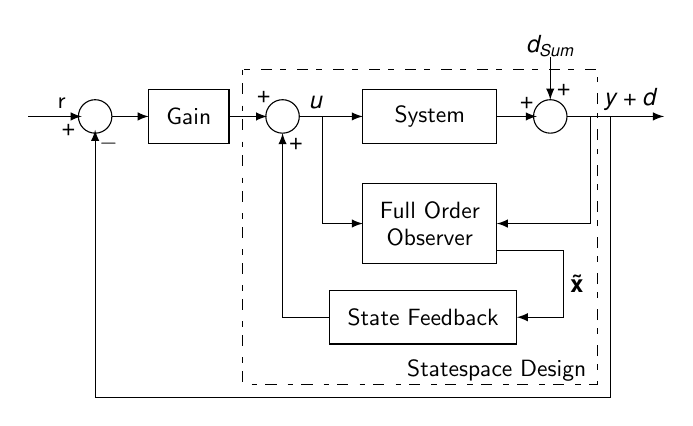
\begin{tikzpicture} [scale=0.85,transform shape]
 \draw [-latex] (-0.2,2) ellipse (0.25 and 0.25);
 \node at (2,2) {\normalsize{System}};
\draw [-latex] (1,2.4) rectangle (3,1.6);
 \node at (2,0.2) {\normalsize{Observer}};
  \node at (2,0.6) {\normalsize{Full Order}};
\draw [-latex] (1,1) rectangle (3,-0.2);
\draw [-latex](0.05,2) -- (1,2);
\draw [-latex](0.4,2) -- (0.4,0.4) -- (1,0.4);
\draw [-latex](4.4,2) -- (4.4,0.4) -- (3,0.4);
 \node at (1.9,-1) {\normalsize{State Feedback}};
\draw [-latex] (0.5,-0.6) rectangle (3.3,-1.4);
  \node at (-1.6,2) {\normalsize{Gain}};
\draw [-latex](-1,2) -- (-0.43,2);
\node at (5,2.25) {\normalsize{$y+d$}};
\node at (0.3,2.2) {\normalsize{$u$}};
\node at (4.2,-0.5) {\normalsize{$\mathbf{\tilde{x}}$}};
\draw [-latex] (-2.2,2.4) rectangle (-1,1.6);
\draw [-latex] (-3,2) ellipse (0.25 and 0.25);
 \draw [-latex] (3.8,2) ellipse (0.25 and 0.25);
\draw [-latex](3,2) -- (3.6,2);
\draw [-latex](4.05,2) -- (5.5,2);
\draw [-latex](-2.75,2) -- (-2.2,2);
\draw [-latex](-4,2) -- (-3.2,2);
\draw [-latex](4.7,2) -- (4.7,-2.2) -- (-3,-2.2) -- (-3,1.8);
 \node at (3.8,3.05) {\normalsize{$d_{Sum}$}};
 \node at (4,2.4) {$+$};
\node at (-2.8,1.6) {$-$};
\node at (-3.4,1.8) {$+$};
\node at (-3.5,2.2) {r };
\draw [dash pattern=on 2pt off 3pt on 4pt off 4pt] (-0.8,2.7) rectangle (4.5,-2);
\node at (3,-1.8) {\normalsize{Statespace Design}};
\node at (-0.48,2.3) {$+$};
\node at (0,1.6) {$+$};
\draw [-latex](0.5,-1) -- (-0.2,-1) -- (-0.2,1.75);
\draw [-latex](3,0) -- (4,0) -- (4,-1) -- (3.3,-1);
\draw [-latex](3.8,2.89) -- (3.8,2.25);
\node at (3.45,2.2) {$+$};
\end{tikzpicture} 
    \vspace{-2mm}
    \captionsetup{font=tiny}
    \captionof{figure}{Block diagram of the control design.}
\end{center}


\end{posterbox}

\begin{posterbox}[name=results_and_simulations,column=1,below=Control]{Results and simulations}

\end{posterbox}

\begin{posterbox}[name=discussion,column=2,below=results]{Discussion}

\end{posterbox}

\begin{posterbox}[name=conclusion,column=2,below=discussion]{Conclusion}

\end{posterbox}

\begin{posterbox}[name=references,column=2,above=bottom]{References}
\bibliography{bibliography}
\end{posterbox}

\end{poster}
\end{document}
